% ! /////////////////////////////
\documentclass[english, a4paper, 11pt]{article}
\usepackage[english]{babel}
\usepackage{microtype}

\usepackage[T1]{fontenc}
\usepackage[utf8]{inputenc}

\usepackage{csquotes}
\usepackage{babel}
\usepackage{pdflscape}
\usepackage{amsmath}
\usepackage{amsfonts}
\usepackage{amssymb}
\usepackage[hidelinks,colorlinks=true,linkcolor=blue,citecolor=blue]{hyperref}
% \usepackage[bookmarks=true]{hyperref}
% \hypersetup{
% 	pdftitle={Testosterone administration and },
% 	pdfauthor={Mohamad Rasoul Parsaeian},
% 	pdfkeywords={Social Hierarchy, single subject design},
% 	bookmarksnumbered,
% 	breaklinks=true,
% 	urlcolor=blue,
% 	citecolor=black,
% 	colorlinks=true,
% 	linkcolor=black,
% }
\usepackage{listings}
\usepackage{lmodern}
\usepackage{amsmath}
\usepackage{amssymb}
\usepackage{textcomp}

\usepackage[style=apa, citestyle=apa]{biblatex}
% \bibliography{references}
% \bibliography{MyLibrary}
\addbibresource{MyLibrary.bib}
% \bibliographystyle{unsrt}
\usepackage[
	per-mode=symbol,
	%output-decimal-marker={,},
	separate-uncertainty=true,
]{siunitx}

\usepackage{booktabs}
\usepackage{caption}
\captionsetup[table]{skip=1ex}

\usepackage{tikz}
\usetikzlibrary{positioning}

\usepackage{graphicx}
\graphicspath{{figures/}}
\usepackage{pgfgantt}

\usepackage[dvipsnames,svgnames,table]{xcolor}
\ganttset{calendar week text={\small{\startday/\startmonth}}}

\usepackage{cleveref}

\usepackage[
    % showframe,
	headheight=16mm,
    bottom=30mm,
]{geometry}

\usepackage{fancyhdr}

\pagestyle{plain}

\usepackage{setspace}

%\usepackage{parskip}

\usepackage{relsize}
\usepackage[nomain, acronym]{glossaries}
\setacronymstyle{long-sm-short}
\newcommand{\newacronymx}[8][]{%
	\newglossaryentry{#2}{
	type=\acronymtype,
	name={{\smaller #3}},
	sort={#3},
	first={#4 ({\smaller #3}, \emph{#5})},
	firstplural={#7 ({\smaller #6}, \emph{#8})},
	text={{\smaller #3}},
	plural={{\smaller #6}},
	description={#4 (\emph{#5})},#1}}

\title{}
\author{}
\date{}

\begin{document}

\begin{center}

    \null\vfill
    \begin{figure}[htp]
        \centering
        
\includegraphics[width=0.4\textwidth]{figures/IPMLogo.png}

    \end{figure}

    {\scshape\large Research Proposal\par}

    \vskip 3\baselineskip

    {\LARGE\bfseries Behavioral and Physiological Consequences of Induced Changes in Social Hierarchies in Male Rats Using the Modified Food Competition Test and Cognitive Modeling via Dynamical Systems Theory: Interplay between Testosterone Administration and Food Access Alterations\par}

    \vskip 3\baselineskip

    By:\\[1ex]
    {\LARGE\bfseries Mohamad Rasoul Parsaeian\par}
    {\small\bfseries m.r.parsa@gmail.com\par}

    \vskip 3\baselineskip

    INSTITUTE FOR RESEARCH
    IN FUNDAMENTAL SCIENCES\\[1ex]
    {\large\bfseries SCHOOL OF COGNITIVE SCIENCE\par}

\end{center}

\vfill

\begin{abstract}
    This research investigates the behavioral and physiological impacts of induced changes in social hierarchies among male rats using an automated system that controls food access through RFID-tagged interactions. Integrating theories such as the frustration-aggression hypothesis (FAH) and dominance hierarchy (DH), we examine how testosterone administration and food access alterations influence social dynamics, aggression, and stress responses within dyads of rats. Control theory principles are employed to design a Social System(SS) where an automated pellet dispenser and testosterone serve as actuators to manipulate or alter social status. Behavioral and physiological data will be collected and analyzed to elucidate the mechanisms underlying social hierarchy formation and maintenance, contributing to the broader understanding of social behavior and its neurobiological foundations.
\end{abstract}

\newpage

\onehalfspacing




\maketitle




\section{Introduction}
Social hierarchy is a complex trait that significantly influences emotion and cognition in both humans and other social species, affecting social organization, survival, reproductive success, and health within groups. Adapting behavior based on social status can be cost-effective and crucial for survival(\cite{vesseyDominanceControl1981}). Typically, social hierarchies are established through aggressive interactions, serving to manage resources and minimize energy expenditure. Once established, hierarchies reduce aggression by organizing priority access to resources. Behavioral paradigms for measuring social hierarchy in lab animals focus on agonistic interactions over scarce resources or territory defense(\cite{zhouAdvancesUnderstandingNeural2018}).

Social hierarchies in rats can be influenced by various factors, including testosterone levels and access to food resources. Testosterone is known to increase aggression and dominance behaviors, while control over food resources can significantly affect social status. The influence of steroid hormones, especially testosterone in males, on aggression has been extensively studied across various species(\cite{hamiltonSocialNeuroendocrinologyStatus2015}). Experimental manipulation of androgenic signaling has shown that these hormones play a causative role in regulating dominance in both males and females. Testosterone is crucial for activating aggressive behavior in the short-term; it peaks during group formation, rises in dominant individuals after aggressive encounters, and can reinforce winner effects(\cite{fuxjagerSpeciesDifferencesWinner2011,oliveiraWhyWinnersKeep2009}).

\section{Background}
A seminal research by O.H. Mowrer aimed to extend behavioral psychology to Marx’s economic theories. The "frustration-aggression" hypothesis was applied to Marx and Engels' analysis of class formation in "The Communist Manifesto," suggesting that Marx's materialist history inadvertently mirrored their psychological system(\cite{dollardFrustrationAggression1939}). The Mowrer and his colleagues  reinterpreted Marx’s theory of class conflict as originating from individual frustration with economic confinement. 
The novel competition test for food rewards has demonstrated stable dominance statuses in adult male rats, providing a robust model for studying the interaction between social hierarchy and stress responses(\cite{costaNovelCompetitionTest2021a})(\Cref{fig:modified_apparatus_feeder},\Cref{fig:modified_apparatus_homecage_reality}).
% Mowrer not only helped theorize this dynamic but also sought to simulate and film its occurrence. In "An Experimentally Produced 'Social Problem' in Rats" (1939)(\cite{nationallibraryofmedicineExperimentallyProducedSocial2021}) and "Competition and Dominance Hierarchies in Rats" (1940)(\cite{paulofranciscoslompCompetitionDominanceHierarchies2011}), he used film to document social interactions and their psychological effects on individual rats. His films focused on the process of individuation, where hierarchies of behavior emerged in groups of rats through multiple experimental interventions, with each rat developing a distinct identity based on its relationship with the group. These films primarily examined the evolution of group dynamics.
\begin{figure}[h]
    \centering
    \begin{tikzpicture}
        % Original image
        \node[inner sep=0pt] (image) at (0,0) {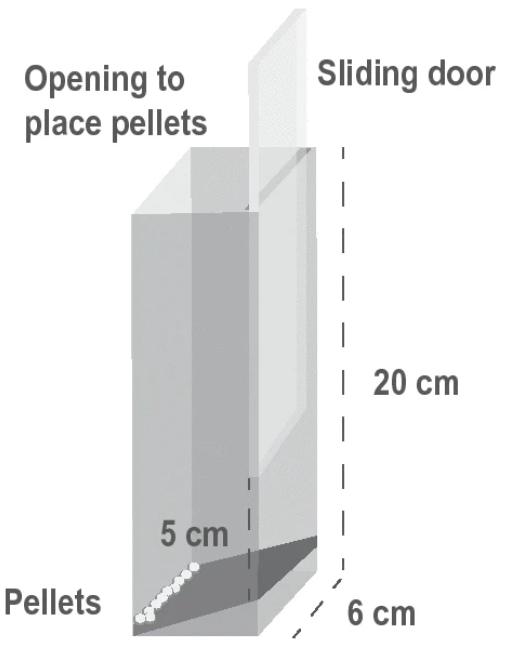
\includegraphics[width=0.8\textwidth]{figures/Feeder.png}};
    \end{tikzpicture}
    \caption{Original Schematic illustration of feeder from \cite{costaNovelCompetitionTest2021a}.}
    \label{fig:modified_apparatus_feeder}
\end{figure}

\begin{figure}[h]
    \centering
    \begin{tikzpicture}
        % Original image
        \node[inner sep=0pt] (image) at (0,0) {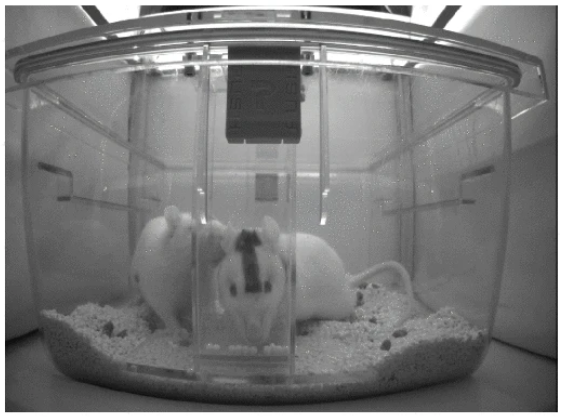
\includegraphics[width=0.8\textwidth]{figures/HomeCageInReality.png}};

    \end{tikzpicture}
    \caption{Original home cage from \cite{costaNovelCompetitionTest2021a}.}
    \label{fig:modified_apparatus_homecage_reality}
\end{figure}
\subsection*{Dynamical Systems and Embedded Cognition in Social Behavior of Animals}

Dynamical systems theory (DST) provides a framework for understanding complex, time-dependent systems through mathematical modeling. In the context of cognition, DST views cognitive processes as dynamic and interactive, continuously evolving over time rather than being static computations. This perspective contrasts with traditional symbolic approaches to cognition, emphasizing the importance of time-dependent interactions within the brain and between the brain, body, and environment(\cite{beerDynamicalSystemsPerspective1995}).

\subsection*{Embedded Cognition}

Embedded cognition is a theory that argues cognitive processes are deeply rooted in the interactions with the environment. This view holds that cognition is not only a result of internal neural processes but also a product of interactions with the physical and social environment. This approach highlights the significance of the situational context in which cognition occurs, suggesting that cognition is inherently tied to the environmental context(\cite{beerDynamicalApproachesCognitive2000}).

\subsection*{Relation to Social Behavior in Animals}

When applied to social behavior in animals, these theories suggest that social interactions and hierarchies are not merely the outcome of internal cognitive processes but are dynamically shaped by continuous interactions with the environment and other animals. In social species, such as rats, these interactions can include competition for resources, communication signals, and physical confrontations, all of which are influenced by the surrounding environment.

In studying social behavior in animals, such as rats, these theories can be applied to understand how social hierarchies form and evolve. For example, the aggression and dominance behaviors seen in rats are not just internal responses but are dynamically influenced by their ongoing interactions with other rats and their environment. This includes the availability of resources, the presence of physical barriers, and the rats' previous experiences.

Understanding social behavior through the lens of dynamical systems and embedded cognition can lead to more effective interventions and experimental designs. For instance, by manipulating the environmental context (e.g., introducing automated food dispensers that respond to specific rats), researchers can observe how these changes affect social hierarchies and individual behaviors over time. This approach offers a comprehensive framework for studying complex social systems in a more holistic manner.




\section{Significance}
This study will provide insights into the mechanisms through which hormonal and environmental factors influence social hierarchies and behavior. The findings will contribute to the understanding of social stress and hierarchy formation in animals.
Understanding the behavioral and physiological impacts of social hierarchy changes in rats can provide insights into social dynamics and stress responses in other social species, including humans. This research could inform interventions for managing social stress and related disorders. This could facilitate organizational social support to be more effective for less privileged groups.  

\section{Experiment Design and Methodology}
\subsection*{Variables}

\subsection*{Independent Variable}
\begin{itemize}
    \item Prioritized access to additional food resources (intervention vs. no intervention).
    \item Dosage of testosterone administration for subordinate rate
\end{itemize}

\subsection*{Dependent Variables}
\begin{itemize}
    \item Social Status
    \item Aggressiveness Level
    \item Corticosterone Level
    \item Testosterone Level
    \item Food Access Level
\end{itemize}
\subsection*{Research Type}

This is an experimental study designed to investigate the behavioral and physiological consequences of induced changes in social hierarchies among dyads of rats.

\subsection*{Research Goals}

\begin{itemize}
    \item To determine the dynamics and procedures of social hierarchy formation in rats.
    \item To assess the impact of prioritized food resource access on subordinate rats.
    \item To monitor behavioral and physiological changes in rats due to altered social hierarchies.
\end{itemize}
\subsection*{Hypotheses}

\begin{itemize}
    \item \textbf{H1}: Subordinate rats given prioritized access to additional food resources will show increased social status over time compared to control rats with the rates proportionate to the dosage of administrated testosterone.
    \item \textbf{H2}: Subordinate rats with prioritized food access will exhibit lower levels of aggressiveness compared to control rats with the rate unproportionate to the dosage of administrated testosterone.
    \item \textbf{H3}: Dominant rats with limited access to food will exhibit higher levels of aggressiveness.
    \item \textbf{H4}: Corticosterone levels will be lower in subordinate rats with additional food access due to reduced stress.
    \item \textbf{H5}: Testosterone levels will increase in subordinate rats with additional food access, correlating with improved social status.
    \item \textbf{H6}: Food access levels will be significantly higher in subordinate rats with the intervention.
\end{itemize}


\subsection*{Participants}
40 adult male Sprague-Dawley rats, housed in groups of 2 (dyads). Rats in each dyad will be matched for their body weight and anxiety level. The anxiety level will be defined by the time spent in the open arms of the Elevated Plus Maze (EPM)(\cite{herreroIndividualDifferencesAnxiety2006,timmerEvidenceRoleOxytocin2011}).




\begin{figure}[h]
    \centering
    \begin{tikzpicture}
        % Original image
        \node[inner sep=0pt] (image) at (0,0) {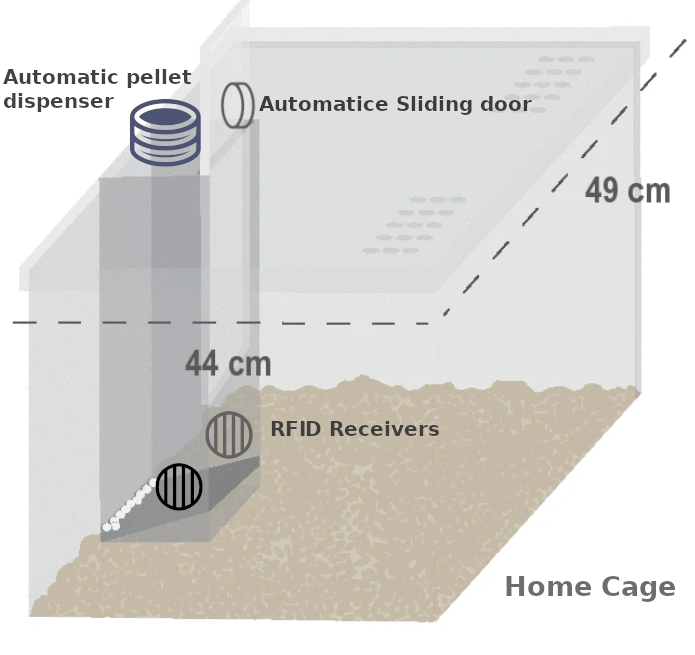
\includegraphics[width=0.8\textwidth]{figures/HomeCageModified.png}};
    \end{tikzpicture}
    \caption{Schematic illustration of the home cage in the modified Food Competition apparatus.}
    \label{fig:modified_apparatus}
\end{figure}


\subsection*{Modified Food Competition Apparatus }

A new version on home cage based on \cite{costaNovelCompetitionTest2021a}(\Cref{fig:modified_apparatus_feeder}) with the following modifications will be developed:
\subsection*{Automated Sliding Door and Pellet Dispenser System}

To study the behavioral and physiological consequences of induced changes in social hierarchies, we will implement an automated system to control access to food resources based on individual rat identification using RFID tags\cite{habedankMouseWhereArt2020}. This system consists of an automatic sliding door and a pellet dispenser, both responsive to RFID tags to ensure only specific rats can access the resources.

\subsubsection*{RFID Tagging}
\begin{itemize}
    \item Each rat is equipped with a unique RFID tag attached to its collar.
    \item The tags are pre-programmed to correspond to the identity of the subordinate or dominant status of each rat.
\end{itemize}

\subsubsection*{Automated Sliding Door}
\begin{itemize}
    \item The sliding door is equipped with a motorized mechanism controlled by a Arduino micro-controller.
    \item An RFID receiver is installed near the sliding door.
    \item When the RFID tag of a subordinate rat is detected by the receiver, the micro-controller activates the motor to open the door, allowing the rat to access the food area.
    \item If the RFID tag of a dominant rat is detected, the door remains closed.
\end{itemize}

\subsubsection*{Pellet Dispenser}
\begin{itemize}
    \item The pellet dispenser is similarly equipped with a motorized mechanism and an RFID receiver.
    \item Upon detecting the RFID tag of the subordinate rat, the dispenser releases a predetermined number of pellets.
    \item The dispenser remains inactive when the RFID tag of the dominant rat is detected, preventing access to additional food resources.
\end{itemize}


\subsection*{Measurement of Variables}

\begin{itemize}
    \item \textbf{Social Status}: Measured by the frequency and outcomes of competitive interactions using the modified Food Competition test and video annotations.
    \item \textbf{Aggressiveness Level}: Assessed using standardized behavioral scoring during interactions using video annotations.
    \item \textbf{Corticosterone Level}: Measured through blood samples at regular intervals.
    \item \textbf{Testosterone Level}: Measured through blood samples at regular intervals.
    \item \textbf{Food Access Level}: Tracked by automated system logs of food dispenser and video annotation.
\end{itemize}

\subsection*{Video annotation}
Bonsai(\cite{lopesBonsaiEventbasedFramework2015}) and Python Video Annotator(\cite{ribeiroPythonvideoannotator}), both open-source computer vision software available online, will be used for behavioral quantification. Initially, Bonsai digitally assigned behaviors and created timestamps for each event's start and end. These timestamps will be then curated frame-by-frame using Python Video Annotator, which allows precise subsecond resolution adjustments. Additionally, Python Video Annotator will enable post hoc categorization of exploration behaviors (anticipatory or resource-present) and pushing behaviors (successful or unsuccessful), which can only be identified after the pushing bouts are completed, making online video analysis insufficient for this purpose.


\section{Experimental Procedure}
\begin{itemize}
    \item \textbf{Baseline Phase}: Initially, the social hierarchy within each dyads of rats is determined using the modified Food Competition test. The dynamics and procedure of hierarchy formation will be recorded
    \item \textbf{Intervention Phase}: The automated system is activated, and the interactions between the rats are monitored. Subordinate rats are given prioritized access to additional food resources through the automated system.
    \item Subordinate rats receive varied dosage of testosterone injections (0.1 mg/kg body weight up to 1 mg/kg body weight every 5 days)(\cite{albertTestosteroneRemovalRats1986,wilsonSocialDominanceCastrate1971}).
    \item \textbf{Monitoring and Data Collection}: Behavioral observations are recorded for 12 weeks, focusing on the frequency and duration of interactions with the sliding door and pellet dispenser. Social hierarchy, agonistic behavior and food consumption will be recorded and measured using video annotations. Physiological measures such as body weight and corticosterone levels are periodically assessed.
\end{itemize}


\section{Expected Outcomes}
\begin{enumerate}
    \item Testosterone administration and food access alterations will lead to significant shifts in social hierarchy.
    \item Combined interventions will result in increased aggression, altered stress responses, and changes in cognitive performance in experiment group but not in control group
    \item The dynamical systems model will accurately predict the effects of these interventions on social hierarchy dynamics.
\end{enumerate}

\section{Schedule of Activities}

The proposed schedule of activities for the project is presented in the Gantt chart in table below.


\newpage

\begin{landscape}
    \begin{figure}[h!bt]
        \begin{center}
            \begin{ganttchart}[
                    hgrid,
                    vgrid={*6{draw=none}, dotted},
                    bar/.append style={fill=black},
                    bar incomplete/.append style={fill=white},
                    time slot format=isodate,
                    time slot format/base century=2000,
                    x unit=0.062cm,
                    y unit chart=0.6cm,
                    y unit title=0.6cm, % height of title line and gap
                    title height=1, % use full height for title, leaving no gap
                    bar top shift=0.1,
                    bar height=0.8,
                    title label font=\bfseries\normalsize,
                    time slot format/start date=2024-10-01]{2024-10-01}{2025-09-28}
                % time slot format/start date=2018-01-01]{2018-01-01}{2018-12-30}
                \gantttitle{Schedule of Activities}{363}\\
                \gantttitlecalendar{year, month=shortname}\\
                %                   increase height   rotate label
                \gantttitlecalendar[title height=1.8, title label node/.append style={rotate=90}]{week}\\
                \gantttitle[title/.style={opacity=0}]{}{364}\\ % invisible title to make room for previous higher line
                % \gantttitle[title/.style={opacity=0}]{}{364}\\ % invisible title to make room for previous higher line
                \ganttbar[bar/.append style={fill=cyan}]{Literature Review}{2024-10-01}{2024-11-15}\\
                \ganttbar[bar/.append style={fill=cyan}]{Tuning Design}{2024-10-01}{2024-12-01}\\
                \ganttbar[bar/.append style={fill=cyan}]{Building Apparatus}{2024-11-02}{2024-12-01}\\
                \ganttbar[bar/.append style={fill=cyan}]{Data Gathering}{2024-12-02}{2025-03-01}\\
                \ganttbar[bar/.append style={fill=cyan}]{Data Analysing}{2025-02-02}{2025-04-01}\\
                \ganttbar[bar/.append style={fill=cyan}]{Draft Paper}{2025-03-15}{2025-05-01}\\
                \ganttbar[bar/.append style={fill=cyan}]{Reviewing Paper}{2025-05-01}{2025-08-01}\\
                \ganttbar[bar/.append style={fill=cyan}]{Submitting Paper}{2025-05-15}{2025-09-28}
            \end{ganttchart}
        \end{center}
        \label{fig:gantt_table}

    \end{figure}
\end{landscape}
\newpage



\section{Data Analysis}
The data collected from the automated system is analyzed to determine changes in social hierarchy dynamics, food access patterns, and physiological responses.
Statistical analyses are performed to compare the behavior and physiological measures between the subordinate and dominant rats in experiment and control groups.





\subsection*{Data Analysis using Repeated Measures ANOVA}

In this section, we describe the process of analyzing changes over time in the experimental data using Repeated Measures ANOVA(\cite{parkCorrectUseRepeated2009}). This statistical method is suitable for comparing the means of three or more groups where the same subjects are used in each group, making it ideal for analyzing longitudinal data from the same group of rats across different time points(\cite{bauerAnalyzingRepeatedMeasures2013a,hershbergerModelingIntraindividualVariability2013a}).

\subsection*{Steps for Data Analysis}

\begin{enumerate}
    \item \textbf{Data Preparation}:
          \begin{itemize}
              \item Ensure the data is structured appropriately, with each row representing a time point and each column representing a measurement for a specific rat.
              \item Organize the data into a format suitable for repeated measures analysis, typically with columns for subject identifiers, time points, and the variable of interest.
          \end{itemize}
    \item \textbf{Statistical Assumptions}:
          \begin{itemize}
              \item Check for sphericity, which is the assumption that the variances of the differences between all combinations of related groups are equal. If sphericity is violated, adjustments such as the Greenhouse-Geisser correction may be applied.
          \end{itemize}
    \item \textbf{Performing Repeated Measures ANOVA}:
          \begin{itemize}
              \item Conduct the ANOVA to test for significant differences over time within subjects.
          \end{itemize}
    \item \textbf{Post-Hoc Analysis}:
          \begin{itemize}
              \item If the ANOVA indicates significant differences, perform post-hoc tests to identify which time points differ from each other.
          \end{itemize}
\end{enumerate}

\subsection*{Python Code for generation test dataset and Repeated Measures ANOVA}

\lstset{language=Python, basicstyle=\ttfamily\footnotesize, keywordstyle=\color{blue}, commentstyle=\color{green}, stringstyle=\color{red}, breaklines=true, frame=single}
\begin{lstlisting}
    import numpy as np
    import pandas as pd
    from scipy.integrate import solve_ivp
    from statsmodels.stats.anova import AnovaRM
    from statsmodels.stats.multicomp import pairwise_tukeyhsd
    import matplotlib.pyplot as plt
    
    # Simulation parameters
    num_rats = 10
    t_points = 50
    np.random.seed(42)
    
    # Simulate time series data
    def simulate_data(num_rats, t_points):
        time = np.arange(t_points)
        data = {
            'Time': np.tile(time, num_rats),
            'Rat': np.repeat(np.arange(num_rats), t_points),
            'Social_Status': np.random.rand(num_rats * t_points),
            'Aggressiveness': np.random.rand(num_rats * t_points),
            'Resource_Access': np.random.rand(num_rats * t_points),
            'Corticosterone': np.random.rand(num_rats * t_points),
            'Testosterone': np.random.rand(num_rats * t_points),
            'Food_Access': np.random.rand(num_rats * t_points)
        }
        return pd.DataFrame(data)
    
    # Generate the data
    df = simulate_data(num_rats, t_points)
    
    # Perform Repeated Measures ANOVA for each attribute
    attributes = ['Social_Status', 'Aggressiveness', 'Resource_Access', 'Corticosterone', 'Testosterone', 'Food_Access']
    
    for attribute in attributes:
        print(f'\nRepeated Measures ANOVA for {attribute}')
        aovrm = AnovaRM(df, attribute, 'Rat', within=['Time'])
        res = aovrm.fit()
        print(res)
    
        # Example of post-hoc analysis (if needed)
        posthoc = pairwise_tukeyhsd(df[attribute], df['Time'])
        print(posthoc)
    
    # Visualizing the simulated data (optional)
    for attribute in attributes:
        plt.figure(figsize=(10, 6))
        for rat in range(num_rats):
            plt.plot(df['Time'][df['Rat'] == rat], df[attribute][df['Rat'] == rat], label=f'Rat {rat}')
        plt.title(f'{attribute} Over Time')
        plt.xlabel('Time')
        plt.ylabel(attribute)
        plt.legend(loc='upper right')
        plt.show()
    
\end{lstlisting}
\subsection*{Dynamic Computational Model}
Based on the hypotheses a model of interactions between variables in regard to time is proposed.  
\subsection*{State Variables}
\begin{itemize}
    \item \( S_i(t) \): Social status of rat \( i \) at time \( t \)
    \item \( A_i(t) \): Aggressiveness level of rat \( i \) at time \( t \)
    \item \( R_i(t) \): Resource access level of rat \( i \) at time \( t \)
    \item \( C_i(t) \): Corticosterone level of rat \( i \) at time \( t \)
    \item \( T_i(t) \): Testosterone level of rat \( i \) at time \( t \)
    \item \( F_i(t) \): Food access level of rat \( i \) at time \( t \)
\end{itemize}

\subsection*{Differential Equations}
\begin{align*}
    \frac{dS_i(t)}{dt} & = \beta A_i(t) + \xi E_i(t) - \eta D_i(t) - \epsilon (S_i(t) - \bar{S}(t)) + \phi T_i(t) + \lambda F_i(t)  \\
    \frac{dA_i(t)}{dt} & = \gamma C_i(t) + \phi T_i(t) - \epsilon (A_i(t) - \bar{A}(t)) + D \frac{\partial^2 A_i(t)}{\partial x^2}  \\
    \frac{dR_i(t)}{dt} & = \alpha S_i(t) - \epsilon (R_i(t) - \bar{R}(t)) + D \frac{\partial^2 R_i(t)}{\partial x^2}                \\
    \frac{dC_i(t)}{dt} & = \frac{1}{1 + \exp(-\theta (R_i(t) - S_i(t)))} - \delta C_i(t) + D \frac{\partial^2 C_i(t)}{\partial x^2} \\
    \frac{dT_i(t)}{dt} & = \text{Testosterone injection rate} - \delta T_i(t) + D \frac{\partial^2 T_i(t)}{\partial x^2}            \\
    \frac{dF_i(t)}{dt} & = \text{Rate of food access} - \delta F_i(t) + D \frac{\partial^2 F_i(t)}{\partial x^2}
\end{align*}


\section*{Model Selection and Fitting}

Model selection and fitting are crucial steps in accurately capturing the dynamics of social hierarchies in rats based on the experimental data. This section describes the process of selecting the appropriate model, fitting the model to the data, and estimating the parameters using Python.

\subsection*{Model Selection}

Model selection involves comparing different models to determine which best describes the observed data. For this experiment, we consider models based on differential equations, such as linear regression, logistic regression, and more complex dynamical systems models.

\subsubsection*{Steps for Model Selection}

\begin{enumerate}
    \item \textbf{Define Candidate Models}
          \begin{itemize}
              \item Linear regression
              \item Logistic regression
              \item Dynamical systems model (e.g., using ordinary differential equations)
          \end{itemize}
    \item \textbf{Model Evaluation Metrics}
          \begin{itemize}
              \item Akaike Information Criterion (AIC)
              \item Bayesian Information Criterion (BIC)
              \item Mean Squared Error (MSE)
              \item R-squared value for goodness-of-fit
          \end{itemize}
    \item \textbf{Cross-Validation}
          \begin{itemize}
              \item Perform k-fold cross-validation to assess model performance on different subsets of data.
          \end{itemize}
\end{enumerate}

\subsection*{Model Fitting and Parameter Estimation}

Once the best model is selected, the next step is fitting the model to the data and estimating the parameters. This involves using optimization techniques to minimize the error between the predicted and observed values.


\subsubsection*{Steps for Model Fitting and Parameter Estimation}

\begin{enumerate}
    \item \textbf{Define the Objective Function}
          \begin{itemize}
              \item The objective function could be the mean squared error between predicted and observed values.
          \end{itemize}
    \item \textbf{Optimization Algorithm}
          \begin{itemize}
              \item Use optimization algorithms such as gradient descent, Newton's method, or more advanced methods like the Levenberg-Marquardt algorithm for non-linear models.
          \end{itemize}
    \item \textbf{Parameter Estimation}
          \begin{itemize}
              \item Estimate the parameters that minimize the objective function.
          \end{itemize}
\end{enumerate}

\subsection*{Python Code for Simulation, Model Selection, Model Fitting, and Parameter Estimation}

\lstset{language=Python, basicstyle=\ttfamily\footnotesize, keywordstyle=\color{blue}, commentstyle=\color{green}, stringstyle=\color{red}, breaklines=true, frame=single}
\begin{lstlisting}
    import numpy as np
    import pandas as pd
    from scipy.integrate import solve_ivp
    from scipy.optimize import minimize
    from sklearn.model_selection import KFold
    from sklearn.metrics import mean_squared_error
    from sklearn.linear_model import LinearRegression
    import matplotlib.pyplot as plt
    
    # Define the testosterone injection rate function
    def testosterone_injection_rate(t, period=5):
        return 1.0 if (t // period) % 2 == 0 else 0.0
    
    # Define the defeat stress exposure rate function
    def defeat_stress_exposure_rate(t, period=5):
        return 1.0 if (t // period) % 2 == 0 else 0.0
    
    # Define the dynamical systems model using ODEs
    def ode_system(t, state, alpha, beta, gamma, delta, epsilon, theta, phi, xi, eta):
        S, A, R, C, T, E, D = state[:7]
        dSdt = beta * A + xi * E - eta * D - epsilon * (S - np.mean(S))
        dAdt = gamma * C + phi * T - epsilon * (A - np.mean(A))
        dRdt = alpha * S - epsilon * (R - np.mean(R))
        dCdt = 1 / (1 + np.exp(-theta * (R - S))) - delta * C
        dTdt = testosterone_injection_rate(t) - delta * T
        dEdt = 0.05 - delta * E
        dDdt = defeat_stress_exposure_rate(t) - delta * D
        return [dSdt, dAdt, dRdt, dCdt, dTdt, dEdt, dDdt]
    
    # Example function to generate synthetic data
    def generate_data(params, num_rats=50, t_points=100):
        initial_conditions = [0.5] * 7
        t = np.linspace(0, 50, t_points)
        sol = solve_ivp(ode_system, [t[0], t[-1]], initial_conditions, t_eval=t, args=params, method='RK45')
        S, A, R, C, T, E, D = sol.y
        return t, S, A, R, C, T, E, D
    
    # Example function for model fitting using optimization
    def fit_model(data, initial_conditions, params_guess):
        def objective_function(params):
            t, S_obs, A_obs, R_obs, C_obs, T_obs, E_obs, D_obs = data
            sol = solve_ivp(ode_system, [t[0], t[-1]], initial_conditions, t_eval=t, args=params, method='RK45')
            S_pred, A_pred, R_pred, C_pred, T_pred, E_pred, D_pred = sol.y
            mse = mean_squared_error(S_obs, S_pred) # Update this line to ensure correct shape
            return mse
    
        result = minimize(objective_function, params_guess, method='L-BFGS-B')
        return result.x
    
    # Example function for model selection using cross-validation
    def model_selection(data, models, scoring):
        kf = KFold(n_splits=5)
        best_model = None
        best_score = float('inf')
    
        for model in models:
            scores = []
            for train_index, test_index in kf.split(data):
                train_data, test_data = data[train_index], data[test_index]
                model.fit(train_data[:, :-1], train_data[:, -1])
                predictions = model.predict(test_data[:, :-1])
                score = scoring(test_data[:, -1], predictions)
                scores.append(score)
    
            avg_score = np.mean(scores)
            if avg_score < best_score:
                best_score = avg_score
                best_model = model
    
        return best_model
    
    # Define candidate models
    models = [
        LinearRegression()
    ]
    
    # Example experimental data
    params = (1.0, 0.5, 0.1, 0.1, 0.05, 2.0, 0.3, 0.2, 0.4)
    t, S, A, R, C, T, E, D = generate_data(params=params, num_rats=50, t_points=100)
    
    # Define initial conditions
    initial_conditions = [0.5] * 7
    
    # Flatten the data for model selection
    data = np.hstack([S[:, np.newaxis], A[:, np.newaxis], R[:, np.newaxis],
                      C[:, np.newaxis], T[:, np.newaxis], E[:, np.newaxis], 
                      D[:, np.newaxis]])
    
    # Model selection using mean squared error
    best_model = model_selection(data, models, scoring=mean_squared_error)
    
    # Fit the selected model to the data
    params_guess = [1.0, 0.5, 0.1, 0.1, 0.05, 2.0, 0.3, 0.2, 0.4]
    best_params = fit_model((t, S, A, R, C, T, E, D), initial_conditions, params_guess)
    
    print("Best Model Parameters:", best_params)
    
\end{lstlisting}


\printbibliography
\end{document}
